 	\documentclass{article}
\usepackage[english]{babel}
\usepackage[utf8]{inputenc}
\usepackage{fancyhdr}
\usepackage{geometry}
\usepackage{enumitem}
\usepackage{amsmath, amssymb}
\usepackage{graphicx}
\usepackage{float}
\usepackage{esdiff}

\geometry{letterpaper, portrait, margin=1in}
\graphicspath{ {images/} }
\pagestyle{fancy}
\fancyhf{}
\lhead{Keerthik Muruganandam}
\rhead{8/15/21 Summer Assignment}
\makeatletter
% This command ignores the optional argument for itemize and enumerate lists
\newcommand{\inlineitem}[1][]{%
\ifnum\enit@type=\tw@
    {\descriptionlabel{#1}}
  \hspace{\labelsep}%
\else
  \ifnum\enit@type=\z@
       \refstepcounter{\@listctr}\fi
    \quad\@itemlabel\hspace{\labelsep}%
\fi}
\makeatother


\begin{document}

\begin{enumerate}[label=\textbf{\arabic*.}]
\item Show that $y=\dfrac{2}{3}e^x+e^{-2x}$ is a solution of the differential equation $y^\prime+2y=2e^x$.\\


\vspace{5pt}
First, $y=\dfrac{2}{3}e^x+e^{-2x}$ be defined as Equation 1, or $(1)$, and $y^\prime+2y=2e^x$ as Equation 2, or $(2)$. Next, the value of $y^\prime$ needs to be found. Because both terms of (1) are very similar to the natural exponential function $e^x$, Equation 1 is relatively simple to differentiate.
\begin{align*}
y &= \frac{2}{3}e^x+e^{-2x}\\
y^\prime &= \frac{2}{3}\diff{}{x}(x)e^x+\diff{ }{x}(-2x)e^{-2x}\\
&= \frac{2}{3}e^x-2e^{-2x}
\end{align*}

Substituting these values for $y^\prime$ and $y$ into Equation 2 provides the new equation:
\[\frac{2}{3}e^x-2e^{-2x} + 2\left(\frac{2}{3}e^x+e^{-2x}\right) =  2e^x\] 
To that Equation 1 is a solution of Equation 2, all that is needed is the simplification of the left hand side of the new equation, which is done below.
\begin{align*}
\frac{2}{3}e^x-2e^{-2x} + 2\left(\frac{2}{3}e^x+e^{-2x}\right) &= \frac{2}{3}e^x-2e^{-2x} +  \frac{4}{3}e^x+2e^{-2x}\\
&= \frac{6}{3}e^x\\
&= 2e^x
\end{align*}
Thus, it has been shown that $y=\dfrac{2}{3}e^x+e^{-2x}$ is a solution of the differential equation $y^\prime+2y=2e^x$.
\newpage

\item Verify that $y = -t\cos t - t$ is a solution of the initial-value problem 
\[t\diff{y}{t} = y+t^2\sin t \;\;\;\;\;\;\;\;\;\;\;\;\;\; y(\pi)=0\]


\vspace{5pt}
Again, the first step is finding the value of $y^\prime$. But before that, the initial value requirement needs to be addressed. The requirement can be validated as follows:
\begin{align*}
y(\pi)&=0\\
-\pi\cos\pi-\pi &= 0\\
&=\pi-\pi\\
&= 0
\end{align*}
Therefore, the initial value is true and the function can be differentiated as follows.
\begin{align*}
y^\prime &= -\diff{}{t}\left(t\cos t+t\right)\\
&= -\left(\diff{}{t}(t)\cos t + \diff{}{t}(\cos t) t\right)-1\\
&= -\cos t +t\sin t-1
\end{align*}
Since the value of $y^\prime$ is now known, simple substitution is all that remains to verify the solution of the problem.
\begin{align*}
y+t^2\sin t &= t\diff{y}{t}\\
&= t\left(-\cos t + t\sin t -1\right)\\
&= -t\cos t+t^2\sin t -t\\
&= \left(-t\cos t-t\right)+t^2\sin t\\
&= y +t^2\sin t
\end{align*}
With this, $y = -t\cos t - t$ has been verified as a solution of the provided initial-value problem.

\newpage 

\item A solution is modeled by the differential equation 
\[\diff{P}{t} = 1.2P\left(1-\dfrac{P}{4200}\right)\]
\begin{enumerate}[label = (\alph*)]
\item For what values is the population increasing?
\item For what values is the population decreasing?
\item What are the equilibrium solutions?
\end{enumerate}


\vspace{5pt}
\begin{enumerate}[label = (\alph*)]
\item This is a very simple problem. The population is increasing when the derivative is positive and vice versa. Therefore, all that needs to be found for this question are the values for which $\diff{P}{t}$ is greater than zero. The eye immediately goes to the expression inside the parentheses, $1-\dfrac{P}{4200}$. It is easily seen that for the derivative to be positive, $P<4200$. The other P in the differential equation creates the lower bound of 0. The values for which the population is increasing are \[(0,4200)\]

\item Using a similar approach to the one used in (a), we just need to find the values of $P$ for which the derivative is negative. First, the P outside of the parentheses ensures that a population below 0 will continually keep decreasing. The expression inside of the parentheses can be used to infer that a population above 4200 will start decreasing because at that point, $1-\dfrac{P}{4200}$ will become negative. The values for which the population is decreasing are \[(-\infty, 0)\cup (4200,\infty)\]

\item We can take the phrase to equilibrium solutions to mean where the value of the derivative is a 0. This only occurs when one of the factors of the differential equation are equal to 0. In this case, the relevant factors are $P$ and $\left(1-\dfrac{P}{4200}\right)$. Some quick mental math results in the values of 0 and 4200 and population values where the population is neither increasing nor decreasing.
\end{enumerate}

\newpage

\item A function $y(t)$ satisfies the differential equation 
\[\diff{y}{t} = y^4-6y^3+5y^2\]
\begin{enumerate}[label = (\alph*)]
\item What are the constant solutions of the equation?
\item For what values of $y$ is $y$ increasing?
\item For what values of $y$ is $y$ decreasing?
\end{enumerate}


\vspace{5pt}
\begin{enumerate}[label = (\alph*)]
\item Using the same approach as the last problem, we simply solve the right hand side for when derivative is in a certain range. For this part, we need to find the solutions for which $\diff{y}{t}$ is 0. This can be solved with some general algebra to yield
\begin{align*}
y^4-6y^3+5y^2 &= y^2(y^2-6y+5)\\
&= y^2(y-5)(y-1)
\end{align*}
Now we can see that the constant solutions are at $y=0, 5, 1$. 

\item To find when $y$ is increasing, the factored form of the differential equation is useful in determining when the derivative is positive. If $y^2(y^2-6y+5)$ is the standard form of the differential equation, $y^2$ can be disregarded because it is always positive. Thus, the only question remaining is when is the $y$ value of the parabola above 0. Because the parabola is positive and the zeroes are at 5 and 1, it is inferred that all value that are not in the interval $(1,5)$ are positive. Thus, $y$ is increasing for the values of $(-\infty,0)\cup(0,1)\cup(5,\infty)$.

\item Using the results from part (b) it is clear that the only values of $y$ for which $y$ is decreasing are $(1,5)$.
\end{enumerate}

\newpage


\item Match the differential equations with the solution graphs labeled I-IV. Give reasons for your choices. 
\begin{enumerate}[label  = (\alph*)]
\item $y^\prime = 1+x^2+y^2$ \qquad\qquad\qquad \inlineitem $y^\prime = xe^{-x^2-y^2}$    \item $y^\prime = \dfrac{1}{1+e^{x^2+y^2}}$ \qquad\qquad\qquad \inlineitem $y^\prime = \sin(xy)\cos(xy)$
\begin{figure}[H]
\centering
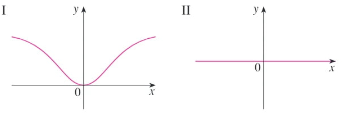
\includegraphics{iii}\\
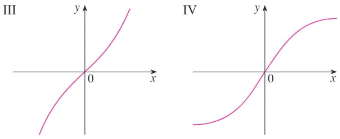
\includegraphics{iiiiv}
\end{figure}
\end{enumerate}

\bigskip

Starting off by analyzing (a), note that the derivative is unbounded and that its solution graph should also reflect that behavior via the curve becoming "steeper" the farther away the point $(x,y)$ on the solution graph is from the origin. The only solution that reflects this behavior is III. \textbf{Therefore, the solution graph of (a) is III.}


Jumping to (d), it is immediately evident that its solution graph is II because the derivative of II must always be 0 no matter what $x$ is, as long as $y=0$. Both (b) and (c) do not fulfill this requirement. For (b) this is because the value of $y$ is only used as an exponent, meaning that even if $y=0$, the value of the overall expression will never be 0. It is the same case for (c). \textbf{Therefore, the solution graph of (d) is II.}

\bigskip

Moving on, the form of (c) is similar to the derivative of $\tan^{-1}(x)$. The solution graph of the latter looks like 
\begin{figure}[H]
\centering
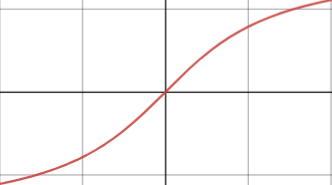
\includegraphics[scale=0.55]{arctan}
\end{figure}
This behavior almost exactly resembles that of IV, suggesting that the solution to (c) is IV. However, we need to confirm. The numerator and denominator of (c), $1$ and $1+e^{x^2+y^2}$, will always be positive no matter the value of $x$ and $y$. In the latter case it is because the exponent of a positive value--$e$--will always return positive. A common pitfall would be to notice that the $y$-value of I is always positive and assume that I is correct. Yet, the \textit{derivative} is positive, not the  output of the equation. What that means graphically is that from left to right, the curve on the graph must always be going up. \textbf{Therefore, the solution graph of (c) is IV.}

\bigskip

Thus, the only solution graph and differential equation left are I and (b). \textbf{Therefore the solution graph of (b) is I.}


\end{enumerate}


\end{document}